\documentclass[10pt,twocolumn]{article}

\usepackage{times}
\usepackage{fullpage}

\renewcommand*\familydefault{times}

\newcommand{\squishlist}{
\begin{list}{$\bullet$}
{ \setlength{\itemsep}{0pt} \setlength{\parsep}{0pt}
\setlength{\topsep}{3pt} \setlength{\partopsep}{0pt}
\setlength{\listparindent}{-2pt}
\setlength{\itemindent}{-5pt}
\setlength{\leftmargin}{0.75em} \setlength{\labelwidth}{0em}
\setlength{\labelsep}{0.5em} } } 
\newcommand{\squishend}{
\end{list} }

\begin{document}

\title{\bf Title}
\author{Paper \# 123}
\date{}
\maketitle
\thispagestyle{empty}


\begin{abstract}

The huge growing performance gap between modern processors and memory ( i.e. the
so called memory wall) is a significant barrier that limits system performance
and hardware caches help mitigate this problem. Sophisticated techniques are
needed now more than ever to better utilize the cache. Cache compression is a
technique that can increase effective cache capacity and reduce misses, improve
performance, and potentially reduce system energy. Hardware compression
algorithms need to be simple in order to reduce the performance overhead as well
as the implementation complexity. The effectiveness of these algorithms are
limited by the layout and range of data in memory. 

The aim of this project is to implement and evaluate compiler optimizations to
improve compressibility of applications’ data in the memory hierarchy.
Specifically we evaluate data structure splitting as a compiler technique to
place data with low relative dynamic range contiguously in memory, thereby
increasing the potential compression ratio when these algorithms are employed.
In this project we implement data structure splitting in LLVM and evaluate the
benefits of our optimization using custom benchmarks. We also explore the
performance impact of this optimization for applications with different data
structure types and memory access patterns and the interaction between cache
locality and data compressibility.

\end{abstract}


\section{Introduction}
\label{sec:intro}

Caches play an important role in modern microprocessors by mitigating the
bandwidth and latency limitations of accessing main memory. Future computer
systems also face power and energy scaling challenges and caches play an
important role in reducing the memory system energy. Hence, it is important to
improve the cache utilization at all levels of the memory hierarchy. 

Cache/memory compression is a technique used to increase on-chip cache capacity
and to decrease on-chip and off-chip bandwidth usage. It is based on the
observation that there is significant redundancy and replication in data stored
either in main memory or in caches which enables storage of data in a more
efficient compressed format. It can be applied using software, hardware or a
combination of both. A key benefit of compression is the increased effective
storage capacity but it also helps reduce off-chip bandwidth and memory traffic
by sending and receiving data in the compressed format. Compression algorithms
like Lempel-Ziv [7] and Base-Delta-Immediate Compression [4] when implemented in
hardware could potentially improve code performance by reducing the number of
long latency accesses to the main memory. There are also potentially significant
power savings by keeping more data in the cache. 

However, there are a few challenges that need to be addressed in order to
effectively exploit these mechanisms. Compression algorithms like
Base-Delta-Immediate Compression leverage patterns, redundancy and similarity in
the data sets. In other words, these algorithms do not work on data with high
dynamic ranges. Another limitation is that the compressibility also depends on
the layout of data in memory. Different data types usually do not compress well
together because the difference in the range of values tend to be very
different. For example. chars, ints, pointers, floats etc. can be expected to
have very different byte sequences in memory. Hardware-based compression is
often effected at the granularity of a cache line. To increase the potential
compression ratio it is desirable that all the data stored in a single cache
line have low dynamic ranges - and, as explained above, similar data types. 

The aim of this project is  to explore compression-conscious data placement
optimizations using the compiler to place data fields with small dynamic ranges
spatially close together in memory. The benefits of these optimizations could
potentially be not only improved compressibility of data in caches and memory
but also simpler logic in the compression hardware. The data layout in memory
usually depends on the choice of data structures used by the programmer. Arrays
of structs are very commonly used to store data sets with disparate fields. A
struct can have many fields with different data types which are placed
contiguously in memory. In these cases the cache line storing the data may not
be very compressible. Also, because of alignment requirements, there is possibly
a lot of wastage of space in the cache line when these data structures are
padded.  

In this project, we evaluate {\em data splitting}  as a compiler technique to
improve the compressibility of data stored in memory. We, however, limit the
scope of our evaluation to cache compression although this compiler optimization
could also potentially aid memory compression. Data splitting involves splitting
a structure with multiple fields into arrays comprising the different fields in
the original data structure. By placing all the data from the same field across
all nodes or structures in a single array.

Figure .. illustrates data splitting and the compressibility benefits. 

There are multiple ways in which splitting data structures may improve
performance. If the program only accesses a few fields frequently at any given
time, placing these hot fields together in memory can actually improve cache
locality and lead to better utilization of the cache and effectively reduces the
working set size, reduces the memory traffic, reduces the number of capacity
misses and does not pollute the cache. Splitting data also creates data streams
that can be prefetched by hardware prefetchers. Most hardware prefetchers can
prefetch from multiple data streams simultaneously and by making the access
pattern more regular, the prefetch accuracy could be potentially higher [1].
Here, we implement and evaluate the benefits of data splitting in generating
data layouts that are more amenable to data compression.

Section details all aspects of our optimization implementation in LLVM. Section
describes the evaluation details including our simulation infrastructure and
testing benchmark.  Section contains a detailed evaluation of our performance
results and experiments.  We discuss related work and future work in Sections ..
and .. and conclude in Section ..

\section{Methodology and Implementation}
\label{sec:meth}

There are three common methods to split structures [1] : { \em affinity based
splitting},  { \em frequency-based splitting} and \em {maximal splitting}. {\em
Affinity-based splitting} typically requires a profiling run to analyze and
determine the affinity of the fields in a structure. Ideally the high affinity
fields should be grouped together while splitting, to ensure that there is no
loss in locality benefits. The structure is then broken down based on the field
affinity. {\em Frequency-based splitting} also needs information about how often
each field is accessed and this can be obtained from a profile or memory trace.
The fields are grouped into frequently-accessed fields, known as hot fields and
infrequently-accessed fields, or cold fields. The structure is split to separate
the {\em hot} and {\em cold fields}. {\em Maximal splitting} does not group any
of the fields in a structure and completely separates all the fields. We
evaluate the impact of splitting and compression with different access patterns,
frequencies (hot vs. cold fields) across a range of cache locality. Due to time
and space constraints we only evaluate maximal splitting. 

Our optimization algorithm functions as follows:

\squishlist

\item Identify all instructions creating arrays of structs.

\item Check if the the structure should be split (currently we use an input file).
Identify the fields in the struct and store the fields and the instruction
generating the fields in a dictionary.

\item Traverse the instruction list, and identify accesses to the data structure. In
LLVM, data structures are accessed using pointers. Some of these are
‘intermediate’ pointers and others are ‘leaf’  pointers which actually point to
the data being accessed.

\item Create a tree from different levels of intermediate pointers and corresponding
leaf pointers.

\item Traverse the pointer tree and compute the corresponding pointers to the new
split arrays.

\item Replace each instruction that generates a pointer with a newly created
instruction that generates the new corresponding pointer as determined above.

\item Replace all uses of a leaf pointer with that of the new leaf pointer
instruction.

\item Traverse the pointer dependence tree above in reverse order and delete all the
old instructions. This is done to ensure that we do not delete an instruction
while it is still being used.

\squishend

Our implementation algorithm ensures that all pointer references at any level of
the overall structure will be redirected to the new split arrays correctly. We
also coalesce multiple pointer computations to reduce the number of these
instructions in generated program. The framework also allows for multiple levels
of nesting with the data structure and enables splitting structures allocated in
the stack, heap as well as global structures. We, however, limit our evaluation
to data structures with a single level of nesting. 

\section{Experimental Setup}
\label{sec:exp}

We use LLVM to implement our proposed optimizations. We also instrumented
Valgrind to evaluate the performance impact of our optimizations.

\subsection{LLVM}
\label{sec:exp-llvm}

We implemented our optimization pass to perform data splitting using LLVM
version 3.4~\cite{llvm}. We do not use any pre-existing libraries or optimization tools
to implement our optimization. 

\subsection{Valgrind}
\label{sec:exp-val}

Valgrind is an instrumentation framework for building dynamic analysis tools. We
evaluate the impact of our optimizations using the cachegrind tool in Valgrind.
Cachegrind simulates how programs interacts with a machine's cache hierarchy. We
altered Valgrind to dynamically compress data using the Base-Delta-Immediate
Compression algorithm while running the program and generate cache hit rates and
data compressibility. 

\subsection{Benchmark}
\label{sec:exp-ben}

In order to evaluate our optimization we wrote a versatile micro-benchmark {\em
structbench}, to enable us to profile the benefits of splitting under different
program behaviors. {\em Structbench} allocates an array of structures in the
{\em stack}, which contains two fields. This micro-benchmark allows us to
specify as input the desired program behaviors that affects benefit for {\em
splitting} and {\em cache compression} including:

\squishlist

\item Field types -- specifies the data types of the two fields of the data
structure. This can affect the benefit we get from {\em splitting} because of
how data is laid out in c/c++ programs. If the sizes of the two fields are
different, unused memory can be inserted into the two fields to ensure the
alignment for the larger field of the two, resulting in internal fragmentation
in the data structure. However, if we split the array of two-field structures
into two arrays, all fields can be laid out contiguously resulting in no
internal fragmentation. This may greatly improve performance of the program
because of the reduced memory footprint potentially making the entire data
structure fit in the processor cache. This can also indirectly affect the
benefit from {\em cache compression} because the value range of the fields is
usually related to the type of the field. For example, an integer field tends to
have values close to zero, while a pointer fields tend to have values relatively
close to each other.

\item Affinity -- specifies the probability of two fields being accessed
together. A higher affinity can potentially negatively affect the benefit we get
from {\em splitting}. A higher affinity indicates that the two fields are more
likely to be accessed together, increasing the spatial locality of the two
fields. However, splitting the data structure breaks the spatial locality.. This
is because the two fields, which were previously located next to each other in
the same cache line, are now separated into two arrays that are distant from
each other.

\item Offset and range -- specifies the offsets of the two fields, and their
ranges compared to their offsets. The benefit from compression can be negatively
impacted if the two fields have offsets that are different from each other, even
if both fields have small value ranges. This is because the two fields, before
splitting, were stored in the same cache line. If the two fields have values
very different from each other, the cache line storing the data structure will
have large dynamic range, making it less compressible. However, if we split the
two fields into two separate arrays, the two fields are not intermingled in the
same cache line. As such, splitting can improve the benefit from cache
compression if the offsets of the two fields are different.

\item Size -- specifies the size of the array. This can inflate or deflate the
benefit we get from both splitting and compression. As described above,
splitting and compression can both potentially help reduce the memory footprint
of the program. This can improve performance because of the reduced memory
accesses. If the size of the array is tuned such that the memory footprint
before splitting and compression, does not fit in the processor cache, but fits
after splitting and compression, the benefit from splitting and compression can
be substantially increased.

\item Access pattern -- specifies the access pattern of the array, ie. whether
the pattern is streaming or random. This can inflate or deflate the benefit we
get from both splitting and compression. This again reduces the memory footprint
of the program, potentially enabling it to fit in the cache. The access pattern
determines if the data is reused or not during the program execution. If the
data is less reused and the data fits in the cache after splitting and
compression, the original program may access memory very frequently, while the
program with data splitting and compression may not.

\squishend



\section{Evaluation}
\label{sec:eval}

We evaluate the benefits of our implementation on our micro-benchmark (described
above) across a range of parameters. We implement the compression algorithm in
the last level of cache. The metrics used for evaluation are the miss rate in
the last level of cache in MPKI and the effective cache capacity increase or
Effective Compression Ratio (ECR) which measures the compressibility of the data
that can actually be utilized with the limitations of hardware implementation.
Figure~\ref{fig:size} shows the benefits of the splitting optimization for different data
set sizes. The miss rate increases with the data set size and the difference in
miss rates between the split vs unsplit structures increases with the size of
the working and stabilizes at higher sizes.  

\begin{figure}[htb]
\centering
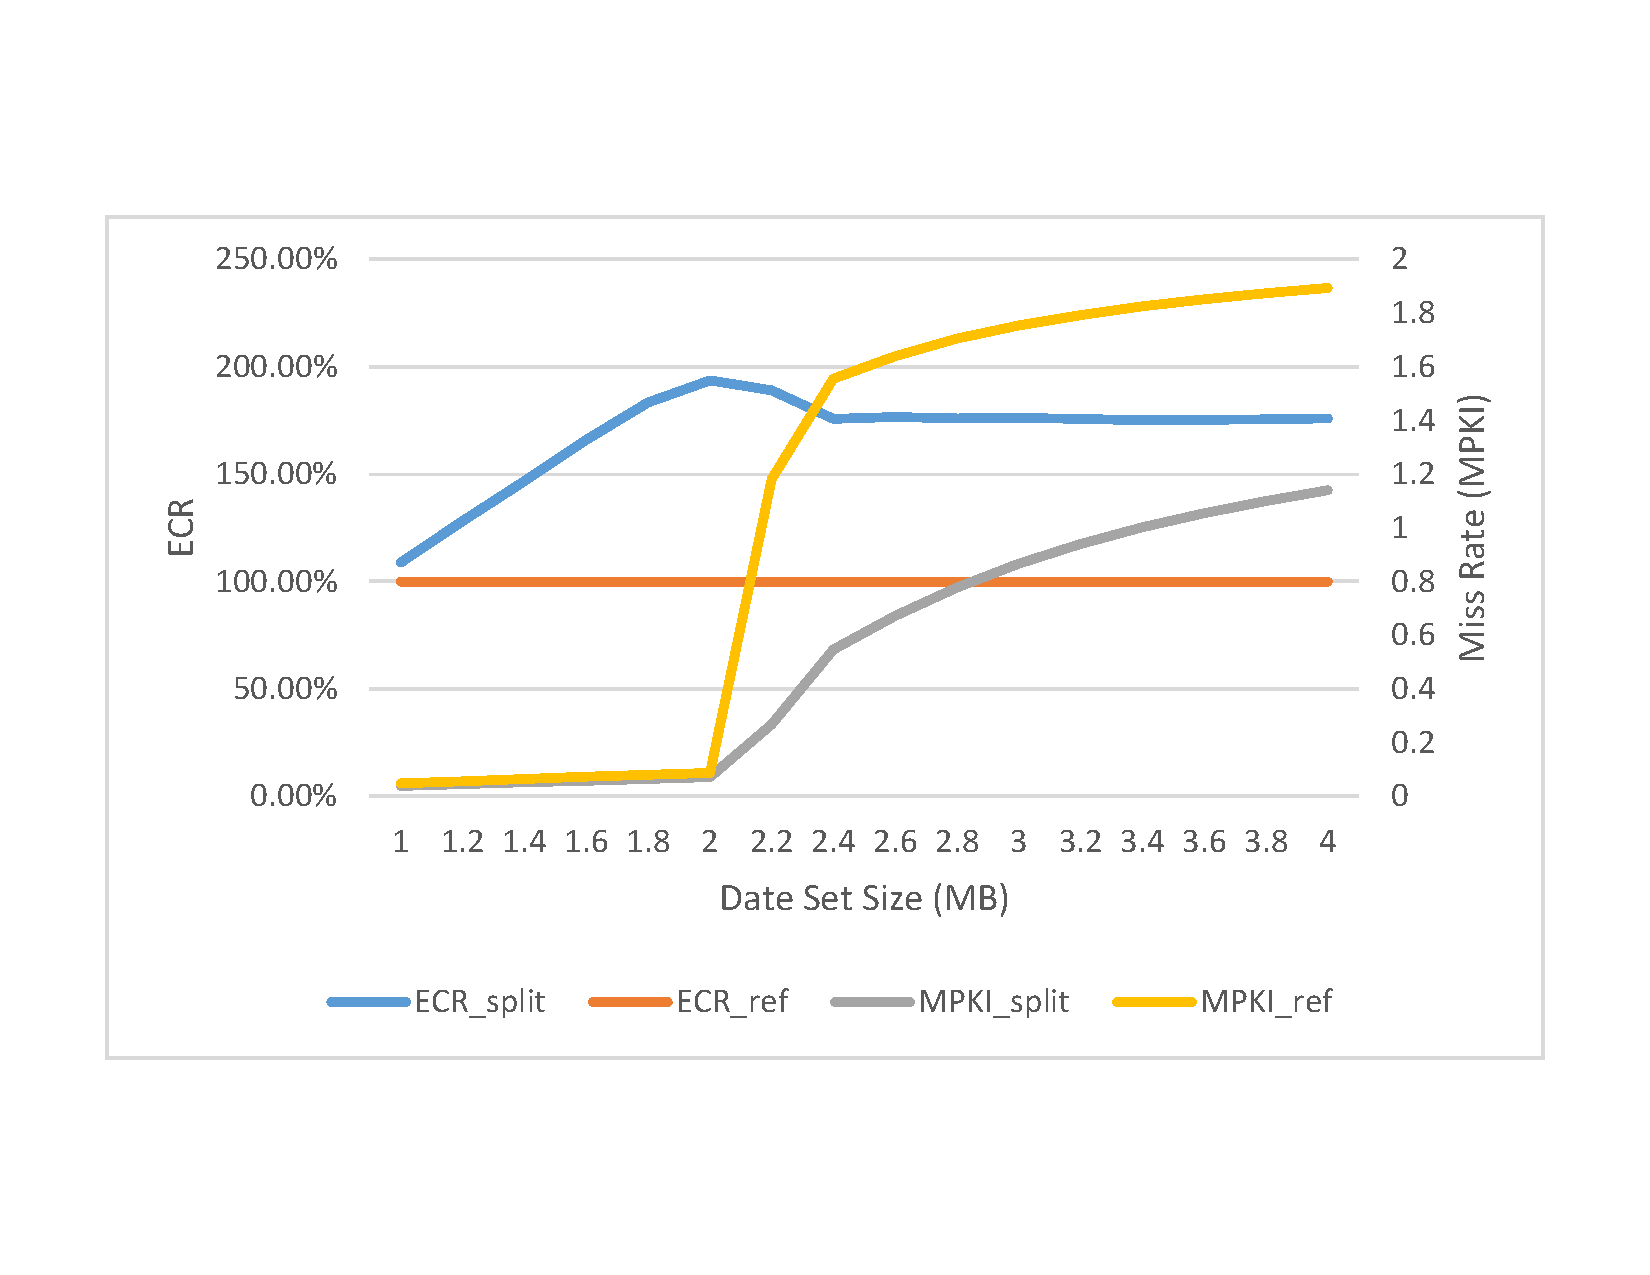
\includegraphics[trim=0mm 0mm 0mm 0mm,clip,width=1\linewidth]{figs/figure2.pdf}
\caption{Effective compression ratio and cache misses per kilo-instructions when
varying the data set size.}
\label{fig:size}
\end{figure}

The splitting benefit for different field affinities is depicted in
Figure~\ref{fig:affinity}.  Here we vary the probability that two fields are
accessed together. In this case we use a random access pattern. There is no
change in compressibility, as expected. As the affinity between the two fields
increases, the miss rate increases when data splitting is employed. This is
because, the benefits from locality outweigh the compression benefits for all
cases except when there is little or no affinity between the fields. The effect
is further exacerbated by the lack of reuse in the data since the access pattern
is random. Figure~\ref{fig:range} shows the variation in compressibility with
differing dynamic ranges. And finally, we evaluate the impact of our
optimization for different field types. We use different combinations of char,
int, float and pointer and illustrate the difference in compressibility and
cache utilization when using data splitting across different field types.
Figure~\ref{type} shows that the impact of data splitting is greatest with
disparate data fields like pointer and char types in the same data structure.
Table~\ref{tbl:field-combinations} maps the different data points in the graph
to the corresponding field combinations. 

\begin{figure}[htb]
\centering
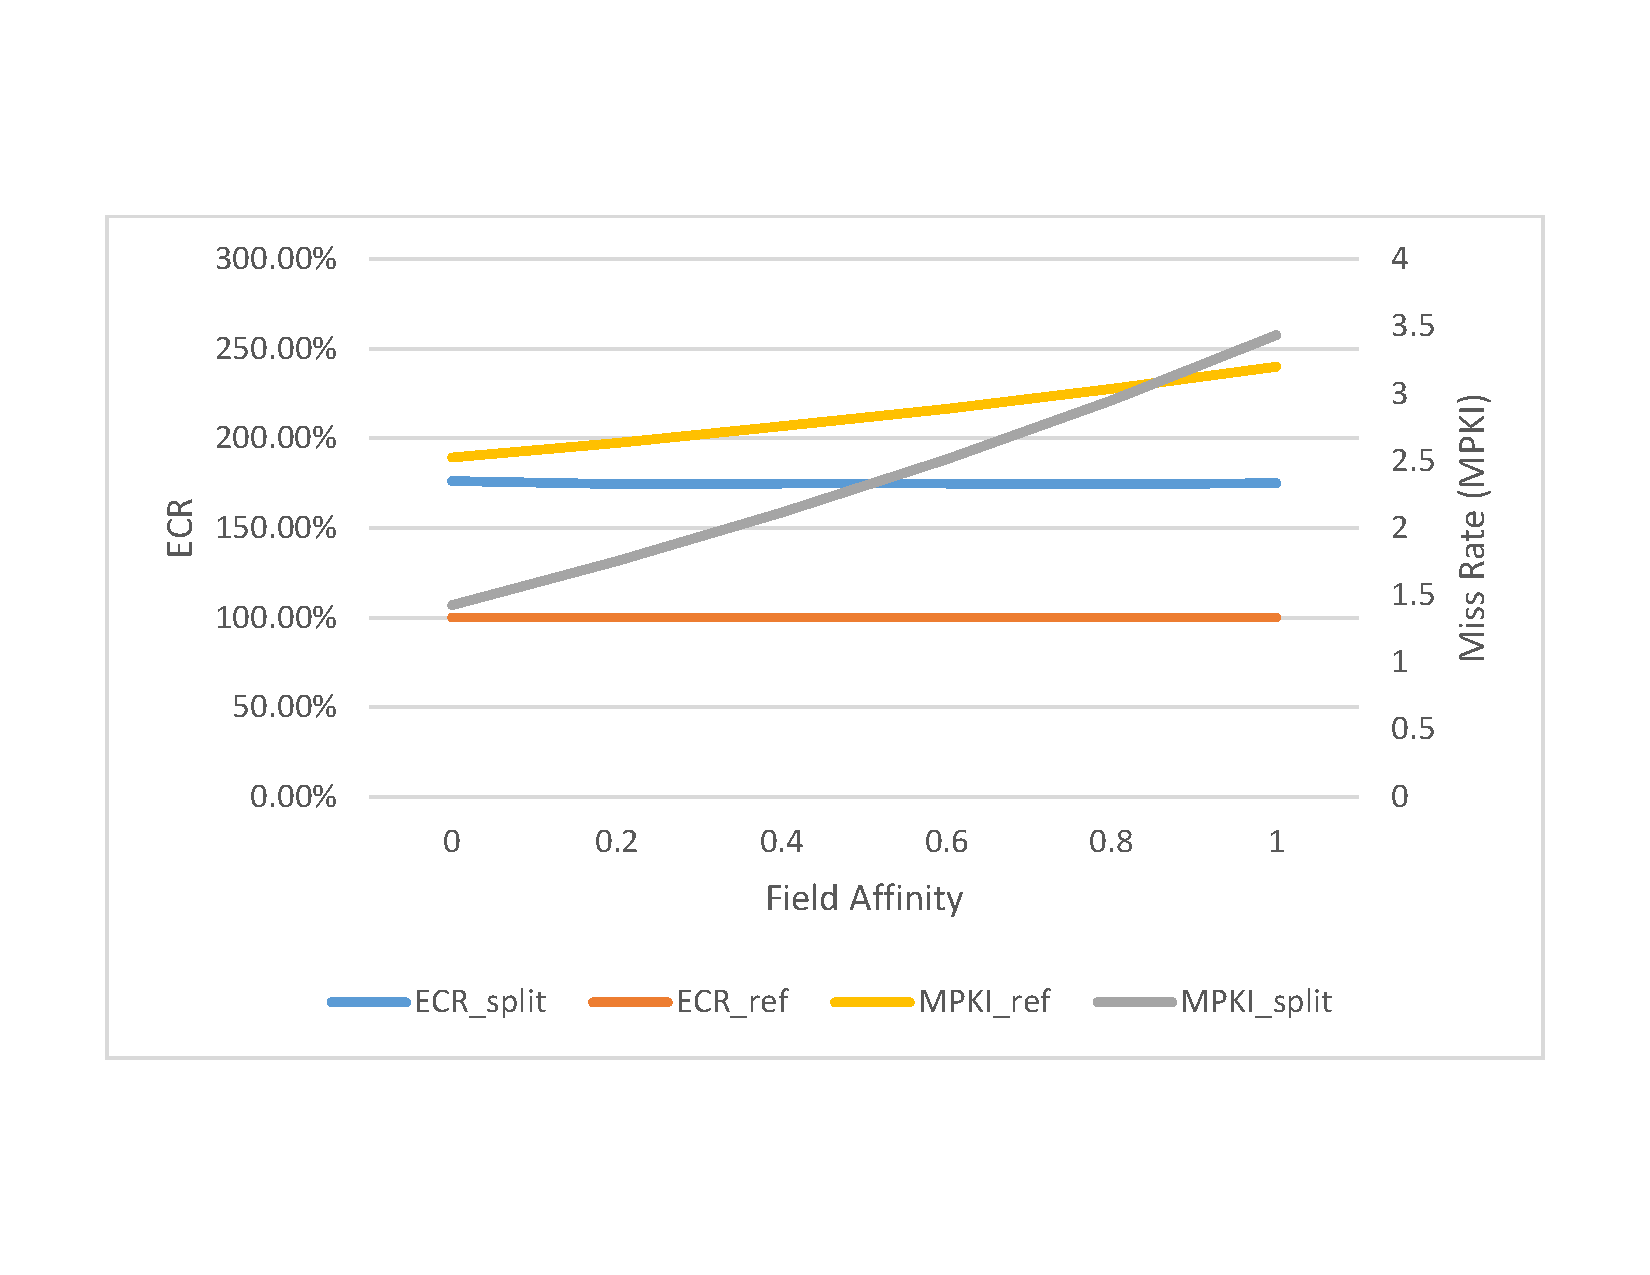
\includegraphics[trim=0mm 0mm 0mm 0mm,clip,width=1\linewidth]{figs/figure.pdf}
\caption{Effective compression ratio and cache misses per kilo-instructions when
varying the affinity value.}
\label{fig:affinity}
\end{figure}

\begin{figure}[htb]
\centering
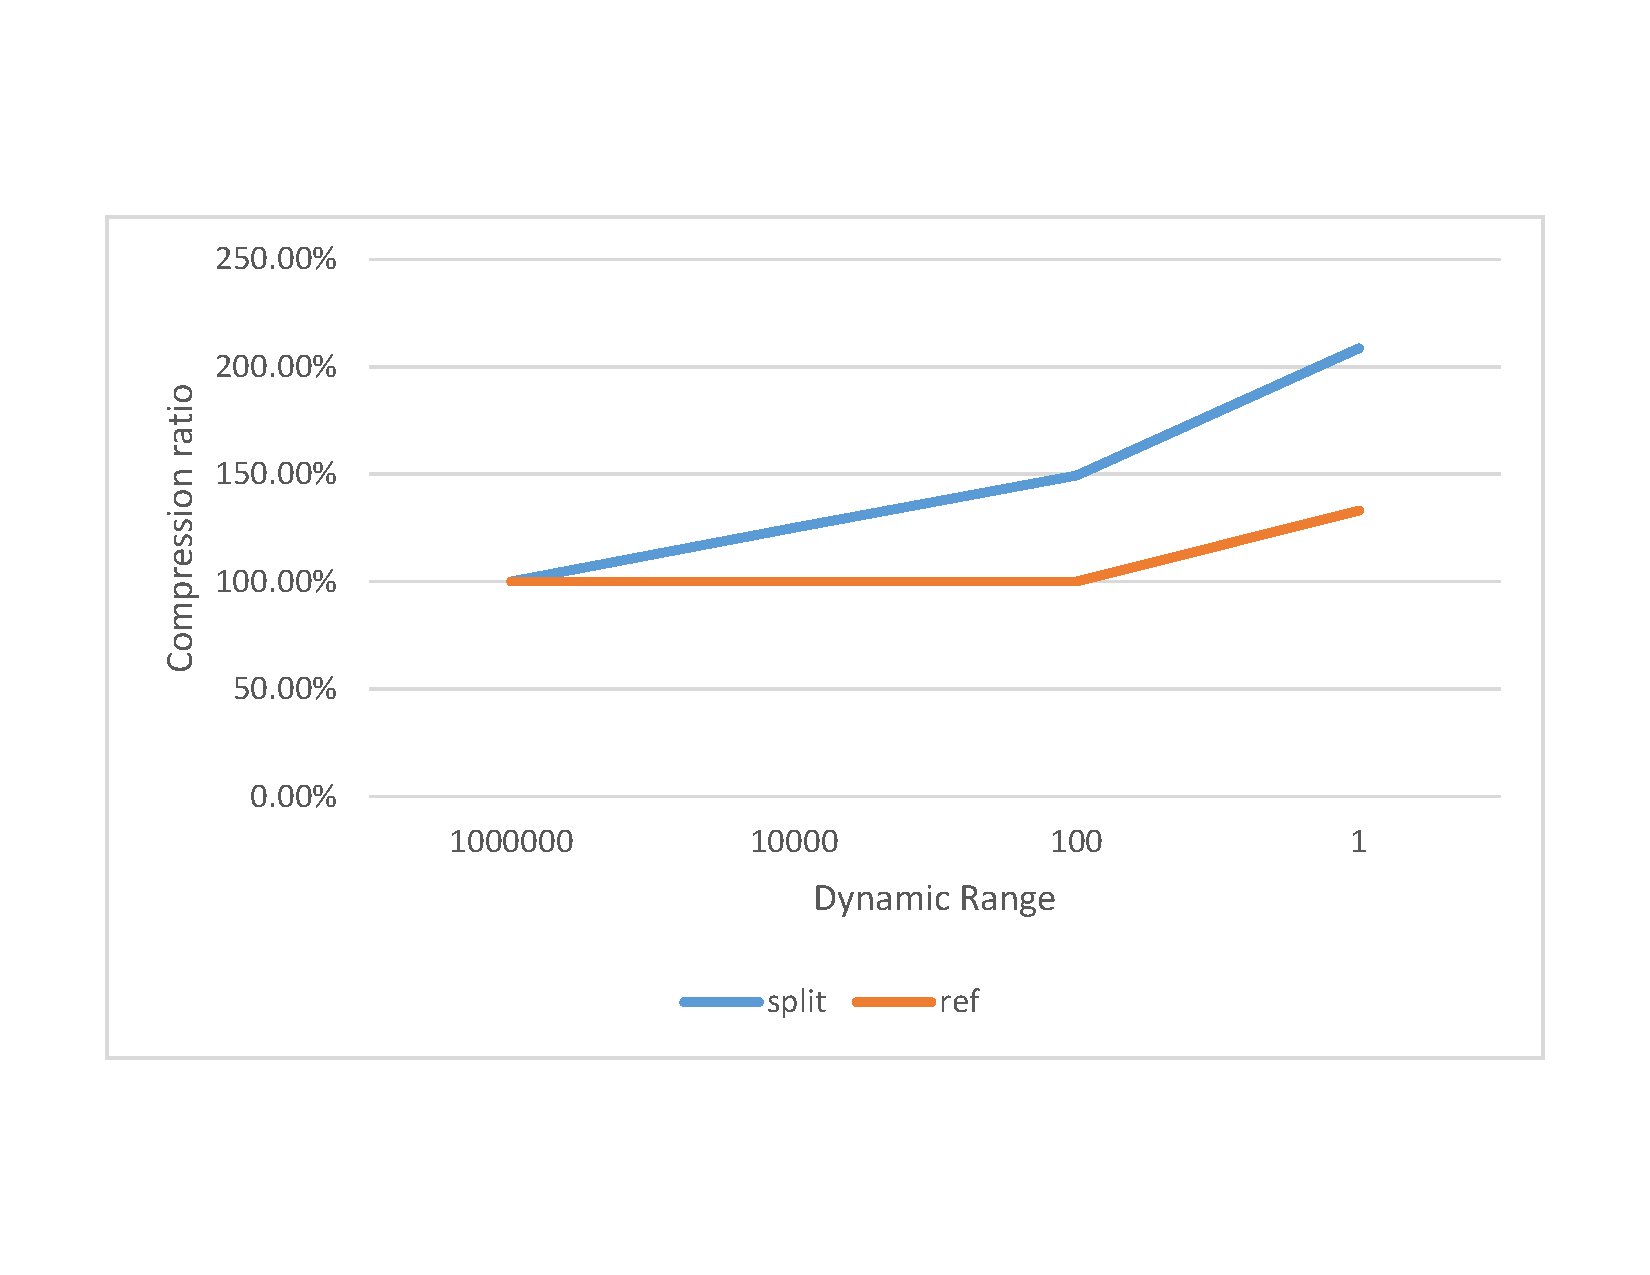
\includegraphics[trim=0mm 0mm 0mm 0mm,clip,width=1\linewidth]{figs/figure3.pdf}
\caption{Effective compression ratio and cache misses per kilo-instructions when
varying the dynamic range.}
\label{fig:range}
\end{figure}

\begin{figure}[htb]
\centering
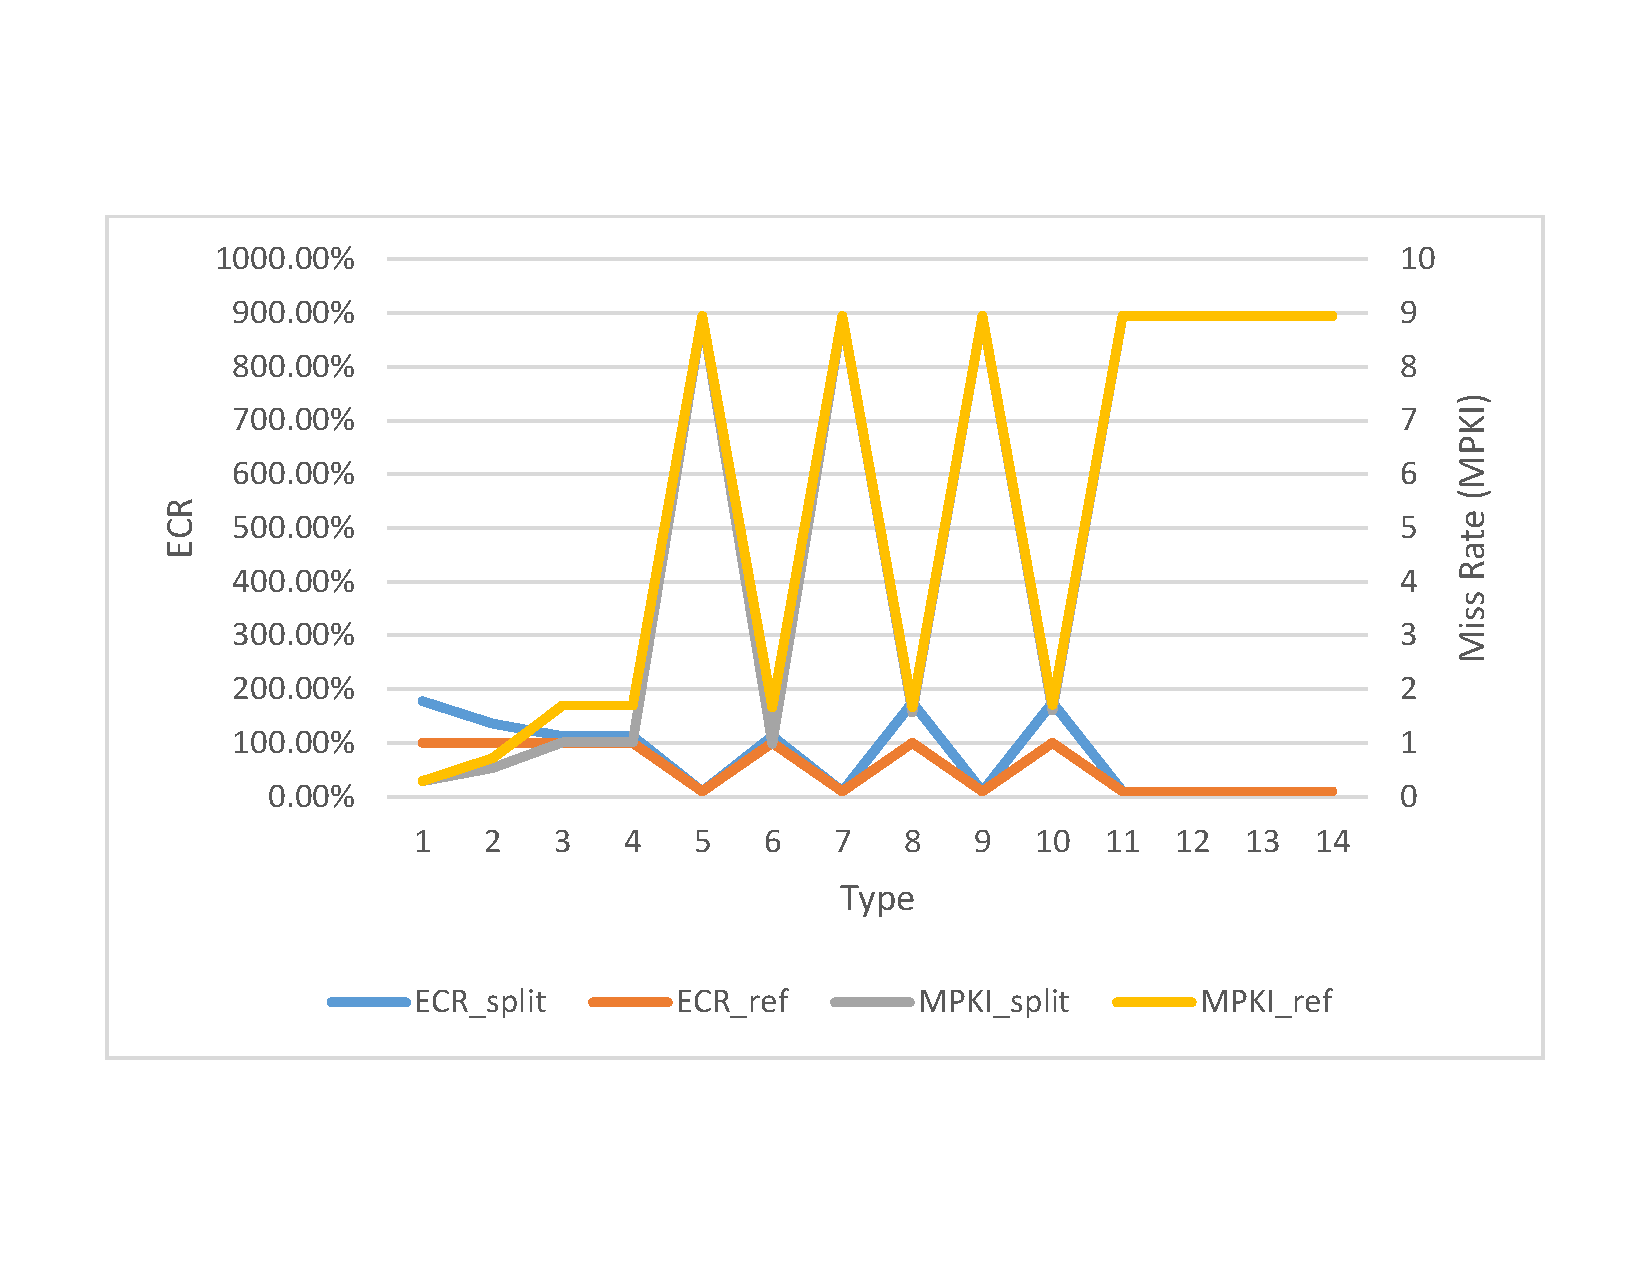
\includegraphics[trim=0mm 0mm 0mm 0mm,clip,width=1\linewidth]{figs/figure4.pdf}
\caption{Effective compression ratio and cache misses per kilo-instructions when
varying the field types.}
\label{fig:type}
\end{figure}

\begin{table}[htb]
\centering
\begin{tabular}{ccc}
\toprule
Label & Field 1 type & Field 2 type \\
\midrule
1 & char & char \\
2 & char & short \\
3 & char & int* \\
4 & char & int \\
5 & char & long long \\
6 & char & float \\
7 & char & double \\
8 & int & float \\
9 & int & double \\
10 & int & int* \\
11 & float & double \\
12 & long long & double \\
13 & long long & float \\
14 & long long & int \\
\bottomrule
\end{tabular}
\caption{Field types combinations.}
\label{tbl:field-combinations}
\end{table}


\section{Related Works}
\label{sec:rel}

Gennady Pekhimenko et. al proposed Base-Delta-Immediate Compression[4]. The key
idea in Base-Delta-Immediate Compression is that data in any cache frequently
have low dynamic range and hence can be compressed with a common base and small
variations or deltas from this base. The authors observe that for many cache
lines, multiple bases are required for efficient compressing due to multi-field
data structures. Trishul Chilimbi et al. proposed Cache-Conscious Structure
Layout[3]. The key idea in Cache-Conscious Structure Layout is that by coloring
and clustering pointers, pointers with spatial locality are grouped together
into a single cache line which improves data reuse. Trishul Chilimbi et al. take
the concept further in Cache-Conscious Structure Definition[2]. In
Cache-Conscious Structure Definition, fields within a structure are further
split into different fields which are reordered to further increase cache
locality and data reuse. Recently, Chris Lattner et al. proposed Automatic Pool
Allocation[5], which segregates heap-based data into separate memory pools and
controls the internal data layout with heuristics. The key idea is to analyze
heap allocated data with a points-to graph and a call graph. Grouping data with
spatial locality together, improves performance. Finally, Stephen Curial
proposed MPADS: Memory-Pooling-Assisted Data Splitting[1], which analyzes
affinity (locality) between fields in a structure and splits data fields based
on their affinity to reduce memory footprint and improve application’s
performance. Fields with low affinity are separated into different pools while
fields with high affinity are bundled together at the granularity of each
element. Memory-Pooling-Assisted Data Splitting improves data reuse by pooling
fields with high affinity while improving memory efficiency by splitting
isolated fields.

\section{Conclusion}
\label{sec:conc}



\section{Future Work}
\label{sec:fut}

As part of our future work, we intend to integrate Memory Pooling with Data
Splitting to enable data splitting in cases where nodes are dynamically
allocated at runtime. We also intend to develop a profiling model based on our
experiments to evaluate the potential benefits from splitting, to detect the
best grouping of fields within a structure and help strike an optimized balance
between locality and compressibility 




\bibliography{refs}
\bibliographystyle{abbrv} 

\end{document}

